% Options for packages loaded elsewhere
\PassOptionsToPackage{unicode}{hyperref}
\PassOptionsToPackage{hyphens}{url}
%
\documentclass[
]{article}
\usepackage{amsmath,amssymb}
\usepackage{iftex}
\ifPDFTeX
  \usepackage[T1]{fontenc}
  \usepackage[utf8]{inputenc}
  \usepackage{textcomp} % provide euro and other symbols
\else % if luatex or xetex
  \usepackage{unicode-math} % this also loads fontspec
  \defaultfontfeatures{Scale=MatchLowercase}
  \defaultfontfeatures[\rmfamily]{Ligatures=TeX,Scale=1}
\fi
\usepackage{lmodern}
\ifPDFTeX\else
  % xetex/luatex font selection
\fi
% Use upquote if available, for straight quotes in verbatim environments
\IfFileExists{upquote.sty}{\usepackage{upquote}}{}
\IfFileExists{microtype.sty}{% use microtype if available
  \usepackage[]{microtype}
  \UseMicrotypeSet[protrusion]{basicmath} % disable protrusion for tt fonts
}{}
\makeatletter
\@ifundefined{KOMAClassName}{% if non-KOMA class
  \IfFileExists{parskip.sty}{%
    \usepackage{parskip}
  }{% else
    \setlength{\parindent}{0pt}
    \setlength{\parskip}{6pt plus 2pt minus 1pt}}
}{% if KOMA class
  \KOMAoptions{parskip=half}}
\makeatother
\usepackage{xcolor}
\usepackage[margin=1in]{geometry}
\usepackage{color}
\usepackage{fancyvrb}
\newcommand{\VerbBar}{|}
\newcommand{\VERB}{\Verb[commandchars=\\\{\}]}
\DefineVerbatimEnvironment{Highlighting}{Verbatim}{commandchars=\\\{\}}
% Add ',fontsize=\small' for more characters per line
\usepackage{framed}
\definecolor{shadecolor}{RGB}{248,248,248}
\newenvironment{Shaded}{\begin{snugshade}}{\end{snugshade}}
\newcommand{\AlertTok}[1]{\textcolor[rgb]{0.94,0.16,0.16}{#1}}
\newcommand{\AnnotationTok}[1]{\textcolor[rgb]{0.56,0.35,0.01}{\textbf{\textit{#1}}}}
\newcommand{\AttributeTok}[1]{\textcolor[rgb]{0.13,0.29,0.53}{#1}}
\newcommand{\BaseNTok}[1]{\textcolor[rgb]{0.00,0.00,0.81}{#1}}
\newcommand{\BuiltInTok}[1]{#1}
\newcommand{\CharTok}[1]{\textcolor[rgb]{0.31,0.60,0.02}{#1}}
\newcommand{\CommentTok}[1]{\textcolor[rgb]{0.56,0.35,0.01}{\textit{#1}}}
\newcommand{\CommentVarTok}[1]{\textcolor[rgb]{0.56,0.35,0.01}{\textbf{\textit{#1}}}}
\newcommand{\ConstantTok}[1]{\textcolor[rgb]{0.56,0.35,0.01}{#1}}
\newcommand{\ControlFlowTok}[1]{\textcolor[rgb]{0.13,0.29,0.53}{\textbf{#1}}}
\newcommand{\DataTypeTok}[1]{\textcolor[rgb]{0.13,0.29,0.53}{#1}}
\newcommand{\DecValTok}[1]{\textcolor[rgb]{0.00,0.00,0.81}{#1}}
\newcommand{\DocumentationTok}[1]{\textcolor[rgb]{0.56,0.35,0.01}{\textbf{\textit{#1}}}}
\newcommand{\ErrorTok}[1]{\textcolor[rgb]{0.64,0.00,0.00}{\textbf{#1}}}
\newcommand{\ExtensionTok}[1]{#1}
\newcommand{\FloatTok}[1]{\textcolor[rgb]{0.00,0.00,0.81}{#1}}
\newcommand{\FunctionTok}[1]{\textcolor[rgb]{0.13,0.29,0.53}{\textbf{#1}}}
\newcommand{\ImportTok}[1]{#1}
\newcommand{\InformationTok}[1]{\textcolor[rgb]{0.56,0.35,0.01}{\textbf{\textit{#1}}}}
\newcommand{\KeywordTok}[1]{\textcolor[rgb]{0.13,0.29,0.53}{\textbf{#1}}}
\newcommand{\NormalTok}[1]{#1}
\newcommand{\OperatorTok}[1]{\textcolor[rgb]{0.81,0.36,0.00}{\textbf{#1}}}
\newcommand{\OtherTok}[1]{\textcolor[rgb]{0.56,0.35,0.01}{#1}}
\newcommand{\PreprocessorTok}[1]{\textcolor[rgb]{0.56,0.35,0.01}{\textit{#1}}}
\newcommand{\RegionMarkerTok}[1]{#1}
\newcommand{\SpecialCharTok}[1]{\textcolor[rgb]{0.81,0.36,0.00}{\textbf{#1}}}
\newcommand{\SpecialStringTok}[1]{\textcolor[rgb]{0.31,0.60,0.02}{#1}}
\newcommand{\StringTok}[1]{\textcolor[rgb]{0.31,0.60,0.02}{#1}}
\newcommand{\VariableTok}[1]{\textcolor[rgb]{0.00,0.00,0.00}{#1}}
\newcommand{\VerbatimStringTok}[1]{\textcolor[rgb]{0.31,0.60,0.02}{#1}}
\newcommand{\WarningTok}[1]{\textcolor[rgb]{0.56,0.35,0.01}{\textbf{\textit{#1}}}}
\usepackage{graphicx}
\makeatletter
\newsavebox\pandoc@box
\newcommand*\pandocbounded[1]{% scales image to fit in text height/width
  \sbox\pandoc@box{#1}%
  \Gscale@div\@tempa{\textheight}{\dimexpr\ht\pandoc@box+\dp\pandoc@box\relax}%
  \Gscale@div\@tempb{\linewidth}{\wd\pandoc@box}%
  \ifdim\@tempb\p@<\@tempa\p@\let\@tempa\@tempb\fi% select the smaller of both
  \ifdim\@tempa\p@<\p@\scalebox{\@tempa}{\usebox\pandoc@box}%
  \else\usebox{\pandoc@box}%
  \fi%
}
% Set default figure placement to htbp
\def\fps@figure{htbp}
\makeatother
\setlength{\emergencystretch}{3em} % prevent overfull lines
\providecommand{\tightlist}{%
  \setlength{\itemsep}{0pt}\setlength{\parskip}{0pt}}
\setcounter{secnumdepth}{-\maxdimen} % remove section numbering
\usepackage{bookmark}
\IfFileExists{xurl.sty}{\usepackage{xurl}}{} % add URL line breaks if available
\urlstyle{same}
\hypersetup{
  pdftitle={Exercícios de Probabilidade},
  pdfauthor={Thierry Martins Ribeiro},
  hidelinks,
  pdfcreator={LaTeX via pandoc}}

\title{Exercícios de Probabilidade}
\author{Thierry Martins Ribeiro}
\date{07/08/2025}

\begin{document}
\maketitle

\begin{Shaded}
\begin{Highlighting}[]
\FunctionTok{library}\NormalTok{(ggplot2)}
\end{Highlighting}
\end{Shaded}

\section{Variaveis}\label{variaveis}

\begin{Shaded}
\begin{Highlighting}[]
\CommentTok{\#X \textasciitilde{} N(90,100) }
\CommentTok{\# 90 = MEDIA}
\CommentTok{\# 100 = VARIANCIA , V\^{}2 = 100 , Variancia = 10}
\end{Highlighting}
\end{Shaded}

\#--------------------------Exercicio 3------------------------------\#

\section{6.3 Exercícios Nos exercícios abaixo iremos também usar o R
como uma calculadora estatística para resolver alguns
exemplos/exercícios de probabilidade tipicamente apresentados em um
curso de estatística básica. Os exercícios abaixo com indicação de
página foram retirados de: Magalhães, M.N. \& Lima, A.C.P. (2001) Noções
de Probabilidade e Estatística. 3 ed.~São Paulo, IME-USP.
392p.}\label{exercuxedcios-nos-exercuxedcios-abaixo-iremos-tambuxe9m-usar-o-r-como-uma-calculadora-estatuxedstica-para-resolver-alguns-exemplosexercuxedcios-de-probabilidade-tipicamente-apresentados-em-um-curso-de-estatuxedstica-buxe1sica.-os-exercuxedcios-abaixo-com-indicauxe7uxe3o-de-puxe1gina-foram-retirados-de-magalhuxe3es-m.n.-lima-a.c.p.-2001-nouxe7uxf5es-de-probabilidade-e-estatuxedstica.-3-ed.-suxe3o-paulo-ime-usp.-392p.}

\begin{Shaded}
\begin{Highlighting}[]
\CommentTok{\#a) P(X \textless{}= 115)}

\NormalTok{solucao\_a }\OtherTok{\textless{}{-}} \FunctionTok{pnorm}\NormalTok{(}\DecValTok{115}\NormalTok{, }\AttributeTok{mean =} \DecValTok{90}\NormalTok{, }\AttributeTok{sd =} \FunctionTok{sqrt}\NormalTok{(}\DecValTok{100}\NormalTok{)) }
\FunctionTok{print}\NormalTok{(solucao\_a)}
\end{Highlighting}
\end{Shaded}

\begin{verbatim}
## [1] 0.9937903
\end{verbatim}

\begin{Shaded}
\begin{Highlighting}[]
\CommentTok{\#b) P(X \textgreater{}= 80)}

\NormalTok{solucao\_b }\OtherTok{\textless{}{-}} \FunctionTok{pnorm}\NormalTok{(}\DecValTok{80}\NormalTok{, }\AttributeTok{mean =} \DecValTok{90}\NormalTok{, }\AttributeTok{sd =} \FunctionTok{sqrt}\NormalTok{(}\DecValTok{100}\NormalTok{))}
\NormalTok{solucao\_b }\OtherTok{\textless{}{-}} \DecValTok{1} \SpecialCharTok{{-}}\NormalTok{ solucao\_b}
\FunctionTok{print}\NormalTok{(solucao\_b)}
\end{Highlighting}
\end{Shaded}

\begin{verbatim}
## [1] 0.8413447
\end{verbatim}

\begin{Shaded}
\begin{Highlighting}[]
\CommentTok{\#c) P(X \textless{}= 75)}

\NormalTok{solucao\_c }\OtherTok{\textless{}{-}} \FunctionTok{pnorm}\NormalTok{(}\DecValTok{75}\NormalTok{, }\AttributeTok{mean =} \DecValTok{90}\NormalTok{, }\AttributeTok{sd =} \FunctionTok{sqrt}\NormalTok{(}\DecValTok{100}\NormalTok{))}
\FunctionTok{print}\NormalTok{(solucao\_c)}
\end{Highlighting}
\end{Shaded}

\begin{verbatim}
## [1] 0.0668072
\end{verbatim}

\begin{Shaded}
\begin{Highlighting}[]
\CommentTok{\#d) P(80 \textless{}= X \textless{}= 110) }

\NormalTok{solucao\_d1 }\OtherTok{\textless{}{-}} \FunctionTok{pnorm}\NormalTok{(}\DecValTok{110}\NormalTok{, }\AttributeTok{mean =} \DecValTok{90}\NormalTok{, }\AttributeTok{sd =} \FunctionTok{sqrt}\NormalTok{(}\DecValTok{100}\NormalTok{))}
\NormalTok{solucao\_d2 }\OtherTok{\textless{}{-}} \FunctionTok{pnorm}\NormalTok{(}\DecValTok{80}\NormalTok{, }\AttributeTok{mean =} \DecValTok{90}\NormalTok{, }\AttributeTok{sd =} \FunctionTok{sqrt}\NormalTok{(}\DecValTok{100}\NormalTok{))}
\NormalTok{solucao\_d }\OtherTok{\textless{}{-}}\NormalTok{ solucao\_d1 }\SpecialCharTok{{-}}\NormalTok{ solucao\_d2}
\FunctionTok{print}\NormalTok{(solucao\_d) }
\end{Highlighting}
\end{Shaded}

\begin{verbatim}
## [1] 0.8185946
\end{verbatim}

\begin{Shaded}
\begin{Highlighting}[]
\CommentTok{\#e) P(|X{-}90| \textless{}= 10)}
\CommentTok{\# |X{-}90| \textless{}= 10 }
\CommentTok{\#1° X {-} 90 \textless{}= 10 =\textgreater{} X \textless{}= 100}
\CommentTok{\#2° {-}(X {-} 90) \textless{}= 10, {-}X + 90 \textless{}= 10, {-}X \textless{}= {-}80, X \textgreater{}= 80}

\NormalTok{solucao\_e1 }\OtherTok{\textless{}{-}} \FunctionTok{pnorm}\NormalTok{(}\DecValTok{100}\NormalTok{, }\AttributeTok{mean =} \DecValTok{90}\NormalTok{, }\AttributeTok{sd =} \FunctionTok{sqrt}\NormalTok{(}\DecValTok{100}\NormalTok{))}
\NormalTok{solucao\_e2 }\OtherTok{\textless{}{-}} \FunctionTok{pnorm}\NormalTok{(}\DecValTok{80}\NormalTok{, }\AttributeTok{mean =} \DecValTok{90}\NormalTok{, }\AttributeTok{sd =} \FunctionTok{sqrt}\NormalTok{(}\DecValTok{100}\NormalTok{))}
\NormalTok{solucao\_e }\OtherTok{\textless{}{-}}\NormalTok{ solucao\_e1 }\SpecialCharTok{{-}}\NormalTok{ solucao\_e2}
\FunctionTok{print}\NormalTok{(solucao\_e)}
\end{Highlighting}
\end{Shaded}

\begin{verbatim}
## [1] 0.6826895
\end{verbatim}

\begin{Shaded}
\begin{Highlighting}[]
\CommentTok{\#f) O valor de alfa tal que $P(90{-}alfa \textless{}= X \textless{}= 90+alfa) = gama, gamma=0.95}

\NormalTok{gama }\OtherTok{\textless{}{-}} \FloatTok{0.95}
\NormalTok{alfa }\OtherTok{\textless{}{-}} \FunctionTok{qnorm}\NormalTok{((}\DecValTok{1} \SpecialCharTok{+}\NormalTok{ gama) }\SpecialCharTok{/} \DecValTok{2}\NormalTok{, }\AttributeTok{mean =} \DecValTok{90}\NormalTok{, }\AttributeTok{sd =} \FunctionTok{sqrt}\NormalTok{(}\DecValTok{100}\NormalTok{)) }\SpecialCharTok{{-}} \DecValTok{90}
\FunctionTok{print}\NormalTok{(alfa)}
\end{Highlighting}
\end{Shaded}

\begin{verbatim}
## [1] 19.59964
\end{verbatim}

\#--------------------------Exercicio 4------------------------------\#

\section{Faça os seguintes
graficos}\label{fauxe7a-os-seguintes-graficos}

\begin{Shaded}
\begin{Highlighting}[]
\CommentTok{\#a) da função de densidade de uma variável com }
\CommentTok{\#distribuição de Poisson com parâmetro $\textbackslash{}lambda = 5$}


\NormalTok{lambda }\OtherTok{\textless{}{-}} \DecValTok{5}
\NormalTok{x }\OtherTok{\textless{}{-}} \DecValTok{0}\SpecialCharTok{:}\DecValTok{10}

\NormalTok{massa }\OtherTok{\textless{}{-}} \FunctionTok{dpois}\NormalTok{(x, lambda)}

\FunctionTok{barplot}\NormalTok{(massa, }\AttributeTok{names.arg =}\NormalTok{ x,}
        \AttributeTok{main =} \StringTok{"Função de Massa de Probabilidade (Poisson λ = 5)"}\NormalTok{,}
        \AttributeTok{xlab =} \StringTok{"k"}\NormalTok{, }\AttributeTok{ylab =} \StringTok{"P(X = k)"}\NormalTok{,}
        \AttributeTok{col =} \StringTok{"lightblue"}\NormalTok{, }\AttributeTok{border =} \StringTok{"blue"}\NormalTok{)}
\end{Highlighting}
\end{Shaded}

\pandocbounded{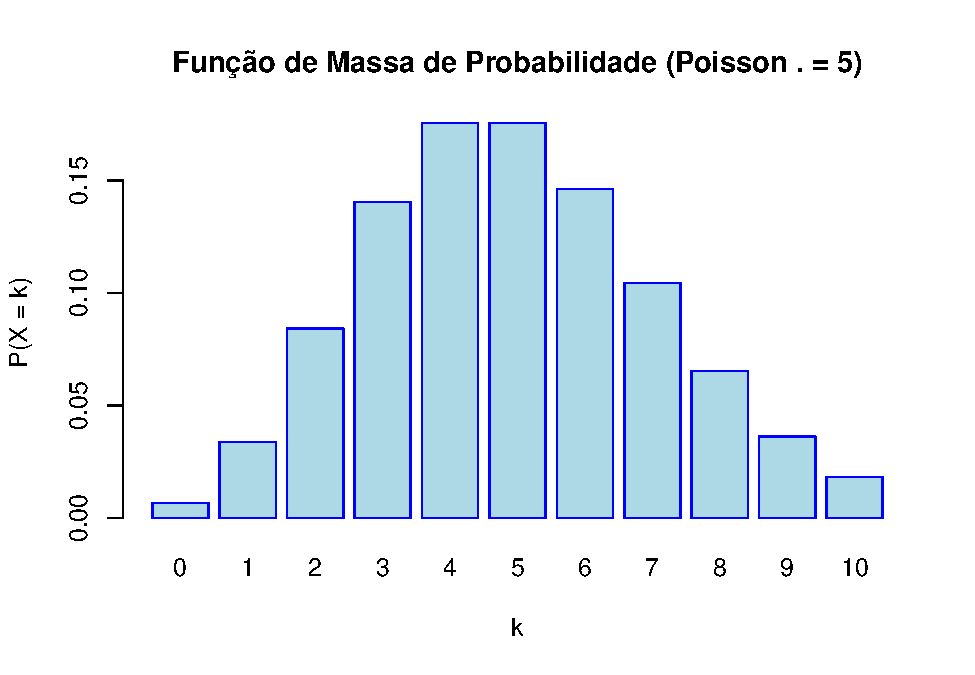
\includegraphics[keepaspectratio]{ex1_files/figure-latex/unnamed-chunk-8-1.pdf}}

\begin{Shaded}
\begin{Highlighting}[]
\CommentTok{\#b) Da densidade de uma variavel X \textasciitilde{} N(90, 100)}


\NormalTok{media }\OtherTok{\textless{}{-}} \DecValTok{90}
\NormalTok{desvio }\OtherTok{\textless{}{-}} \DecValTok{10}

\NormalTok{x }\OtherTok{\textless{}{-}} \FunctionTok{seq}\NormalTok{(}\DecValTok{60}\NormalTok{, }\DecValTok{120}\NormalTok{, }\AttributeTok{by =} \FloatTok{0.1}\NormalTok{)}

\NormalTok{densidade }\OtherTok{\textless{}{-}} \FunctionTok{dnorm}\NormalTok{(x, }\AttributeTok{mean =}\NormalTok{ media, }\AttributeTok{sd =}\NormalTok{ desvio)}

\FunctionTok{plot}\NormalTok{(x, densidade, }\AttributeTok{type =} \StringTok{"l"}\NormalTok{, }\AttributeTok{lwd =} \DecValTok{2}\NormalTok{,}
     \AttributeTok{main =} \StringTok{"Função de Densidade da Normal N(90, 100)"}\NormalTok{,}
     \AttributeTok{xlab =} \StringTok{"x"}\NormalTok{, }\AttributeTok{ylab =} \StringTok{"f(x)"}\NormalTok{,}
     \AttributeTok{col =} \StringTok{"darkgreen"}\NormalTok{)}
\end{Highlighting}
\end{Shaded}

\pandocbounded{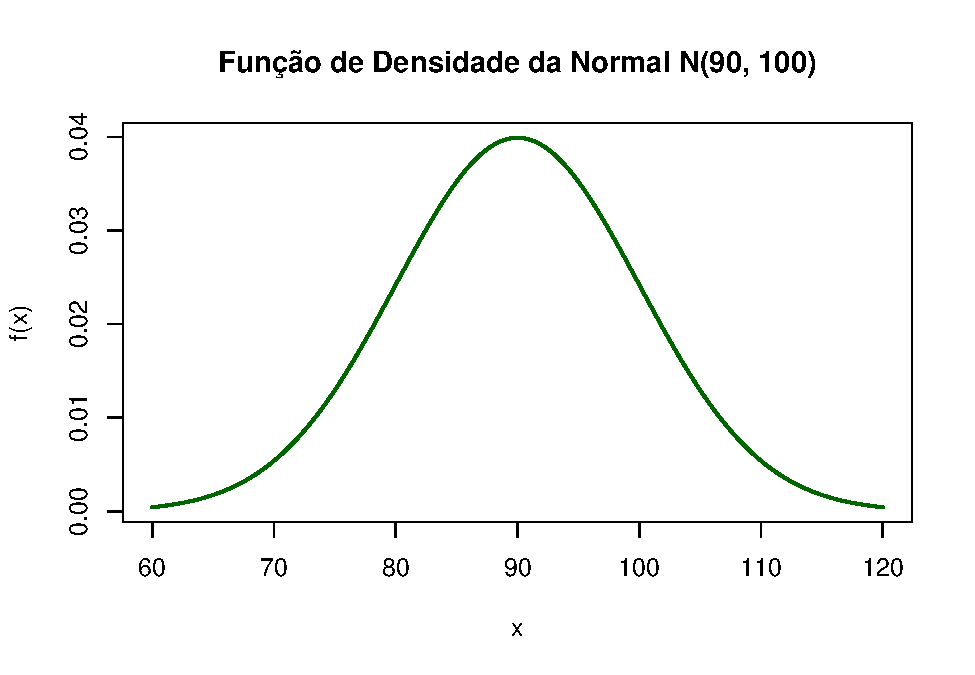
\includegraphics[keepaspectratio]{ex1_files/figure-latex/unnamed-chunk-9-1.pdf}}

\begin{Shaded}
\begin{Highlighting}[]
\CommentTok{\#c) sobreponha ao gráfico anterior a densidade de uma variável }
\CommentTok{\#$Y \textbackslash{}sim N(90, 80)$ e outra $Z \textbackslash{}sim N(85, 100)$}


\NormalTok{x }\OtherTok{\textless{}{-}} \FunctionTok{seq}\NormalTok{(}\DecValTok{50}\NormalTok{, }\DecValTok{130}\NormalTok{, }\AttributeTok{by =} \FloatTok{0.1}\NormalTok{)}


\NormalTok{densidade\_X }\OtherTok{\textless{}{-}} \FunctionTok{dnorm}\NormalTok{(x, }\AttributeTok{mean =} \DecValTok{90}\NormalTok{, }\AttributeTok{sd =} \FunctionTok{sqrt}\NormalTok{(}\DecValTok{100}\NormalTok{))     }
\NormalTok{densidade\_Y }\OtherTok{\textless{}{-}} \FunctionTok{dnorm}\NormalTok{(x, }\AttributeTok{mean =} \DecValTok{90}\NormalTok{, }\AttributeTok{sd =} \FunctionTok{sqrt}\NormalTok{(}\DecValTok{80}\NormalTok{))      }
\NormalTok{densidade\_Z }\OtherTok{\textless{}{-}} \FunctionTok{dnorm}\NormalTok{(x, }\AttributeTok{mean =} \DecValTok{85}\NormalTok{, }\AttributeTok{sd =} \FunctionTok{sqrt}\NormalTok{(}\DecValTok{100}\NormalTok{))     }

\FunctionTok{plot}\NormalTok{(x, densidade\_X, }\AttributeTok{type =} \StringTok{"l"}\NormalTok{, }\AttributeTok{lwd =} \DecValTok{2}\NormalTok{, }\AttributeTok{col =} \StringTok{"blue"}\NormalTok{,}
     \AttributeTok{ylim =} \FunctionTok{c}\NormalTok{(}\DecValTok{0}\NormalTok{, }\FunctionTok{max}\NormalTok{(densidade\_X, densidade\_Y, densidade\_Z)),}
     \AttributeTok{main =} \StringTok{"Densidades de X \textasciitilde{} N(90,100), Y \textasciitilde{} N(90,80) e Z \textasciitilde{} N(85,100)"}\NormalTok{,}
     \AttributeTok{xlab =} \StringTok{"x"}\NormalTok{, }\AttributeTok{ylab =} \StringTok{"f(x)"}\NormalTok{)}


\FunctionTok{lines}\NormalTok{(x, densidade\_Y, }\AttributeTok{col =} \StringTok{"red"}\NormalTok{, }\AttributeTok{lwd =} \DecValTok{2}\NormalTok{, }\AttributeTok{lty =} \DecValTok{2}\NormalTok{)}

\FunctionTok{lines}\NormalTok{(x, densidade\_Z, }\AttributeTok{col =} \StringTok{"darkgreen"}\NormalTok{, }\AttributeTok{lwd =} \DecValTok{2}\NormalTok{, }\AttributeTok{lty =} \DecValTok{3}\NormalTok{)}

\FunctionTok{legend}\NormalTok{(}\StringTok{"topright"}\NormalTok{, }\AttributeTok{legend =} \FunctionTok{c}\NormalTok{(}\StringTok{"X \textasciitilde{} N(90, 100)"}\NormalTok{, }\StringTok{"Y \textasciitilde{} N(90, 80)"}\NormalTok{, }\StringTok{"Z \textasciitilde{} N(85, 100)"}\NormalTok{),}
       \AttributeTok{col =} \FunctionTok{c}\NormalTok{(}\StringTok{"blue"}\NormalTok{, }\StringTok{"red"}\NormalTok{, }\StringTok{"darkgreen"}\NormalTok{), }\AttributeTok{lwd =} \DecValTok{2}\NormalTok{, }\AttributeTok{lty =} \FunctionTok{c}\NormalTok{(}\DecValTok{1}\NormalTok{, }\DecValTok{2}\NormalTok{, }\DecValTok{3}\NormalTok{))}
\end{Highlighting}
\end{Shaded}

\pandocbounded{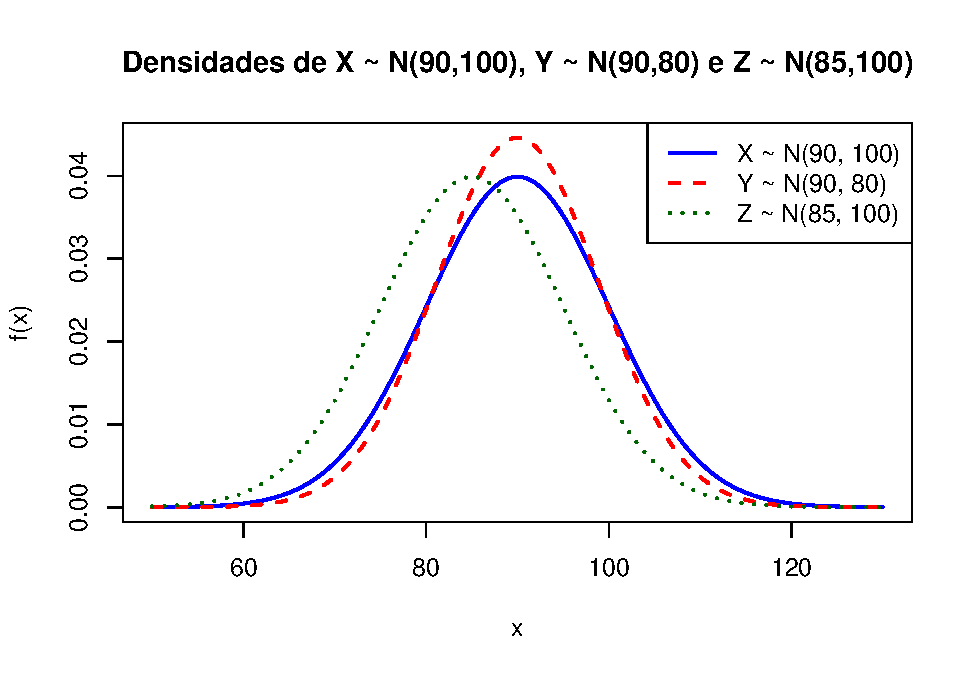
\includegraphics[keepaspectratio]{ex1_files/figure-latex/unnamed-chunk-10-1.pdf}}

\begin{Shaded}
\begin{Highlighting}[]
\CommentTok{\#d) densidades de distribuições }
\CommentTok{\#$\textbackslash{}chi\^{}2$ com 1, 2 e 5 graus de liberdade.}

\NormalTok{x }\OtherTok{\textless{}{-}} \FunctionTok{seq}\NormalTok{(}\DecValTok{0}\NormalTok{, }\DecValTok{20}\NormalTok{, }\AttributeTok{by =} \FloatTok{0.1}\NormalTok{)}

\NormalTok{dens\_1 }\OtherTok{\textless{}{-}} \FunctionTok{dchisq}\NormalTok{(x, }\AttributeTok{df =} \DecValTok{1}\NormalTok{)}
\NormalTok{dens\_2 }\OtherTok{\textless{}{-}} \FunctionTok{dchisq}\NormalTok{(x, }\AttributeTok{df =} \DecValTok{2}\NormalTok{)}
\NormalTok{dens\_5 }\OtherTok{\textless{}{-}} \FunctionTok{dchisq}\NormalTok{(x, }\AttributeTok{df =} \DecValTok{5}\NormalTok{)}


\NormalTok{all\_dens }\OtherTok{\textless{}{-}} \FunctionTok{c}\NormalTok{(dens\_1, dens\_2, dens\_5)}
\NormalTok{all\_dens }\OtherTok{\textless{}{-}}\NormalTok{ all\_dens[}\FunctionTok{is.finite}\NormalTok{(all\_dens)]}

\FunctionTok{plot}\NormalTok{(x, dens\_1, }\AttributeTok{type =} \StringTok{"l"}\NormalTok{, }\AttributeTok{lwd =} \DecValTok{2}\NormalTok{, }\AttributeTok{col =} \StringTok{"blue"}\NormalTok{,}
     \AttributeTok{ylim =} \FunctionTok{c}\NormalTok{(}\DecValTok{0}\NormalTok{, }\FunctionTok{max}\NormalTok{(all\_dens)),}
     \AttributeTok{main =} \StringTok{"Densidades da distribuição χ² com 1, 2 e 5 graus de liberdade"}\NormalTok{,}
     \AttributeTok{xlab =} \StringTok{"x"}\NormalTok{, }\AttributeTok{ylab =} \StringTok{"f(x)"}\NormalTok{)}


\FunctionTok{lines}\NormalTok{(x, dens\_2, }\AttributeTok{col =} \StringTok{"red"}\NormalTok{, }\AttributeTok{lwd =} \DecValTok{2}\NormalTok{, }\AttributeTok{lty =} \DecValTok{2}\NormalTok{)}
\FunctionTok{lines}\NormalTok{(x, dens\_5, }\AttributeTok{col =} \StringTok{"darkgreen"}\NormalTok{, }\AttributeTok{lwd =} \DecValTok{2}\NormalTok{, }\AttributeTok{lty =} \DecValTok{3}\NormalTok{)}

\FunctionTok{legend}\NormalTok{(}\StringTok{"topright"}\NormalTok{, }\AttributeTok{legend =} \FunctionTok{c}\NormalTok{(}\StringTok{"χ²(1)"}\NormalTok{, }\StringTok{"χ²(2)"}\NormalTok{, }\StringTok{"χ²(5)"}\NormalTok{),}
       \AttributeTok{col =} \FunctionTok{c}\NormalTok{(}\StringTok{"blue"}\NormalTok{, }\StringTok{"red"}\NormalTok{, }\StringTok{"darkgreen"}\NormalTok{), }\AttributeTok{lwd =} \DecValTok{2}\NormalTok{, }\AttributeTok{lty =} \FunctionTok{c}\NormalTok{(}\DecValTok{1}\NormalTok{, }\DecValTok{2}\NormalTok{, }\DecValTok{3}\NormalTok{))}
\end{Highlighting}
\end{Shaded}

\pandocbounded{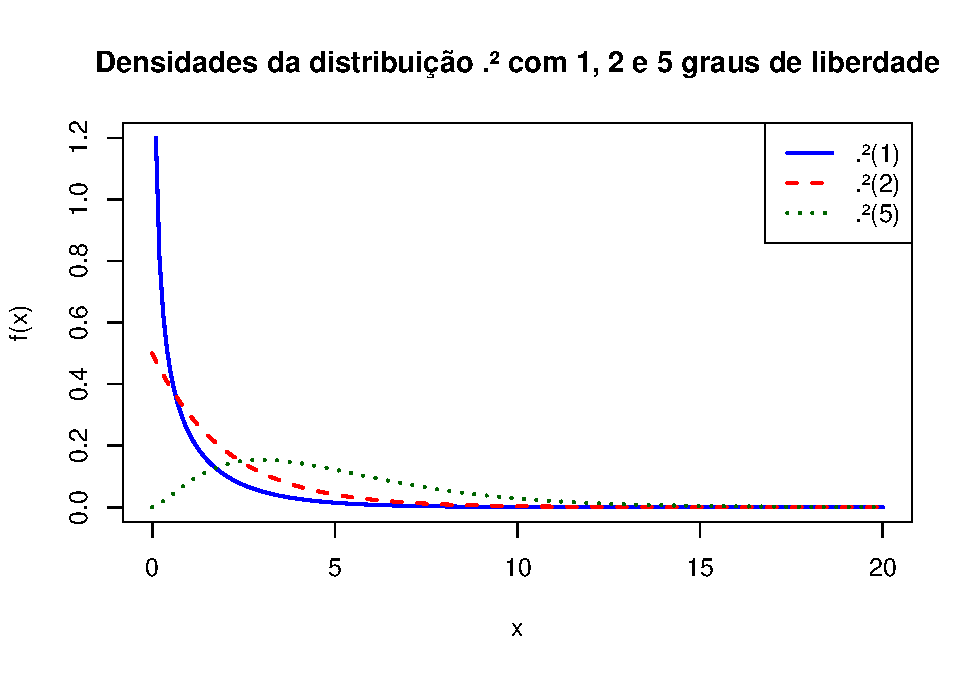
\includegraphics[keepaspectratio]{ex1_files/figure-latex/unnamed-chunk-11-1.pdf}}

\end{document}
